\documentclass{standalone}
\usepackage{tikz}
\usetikzlibrary{patterns, positioning}

\begin{document}
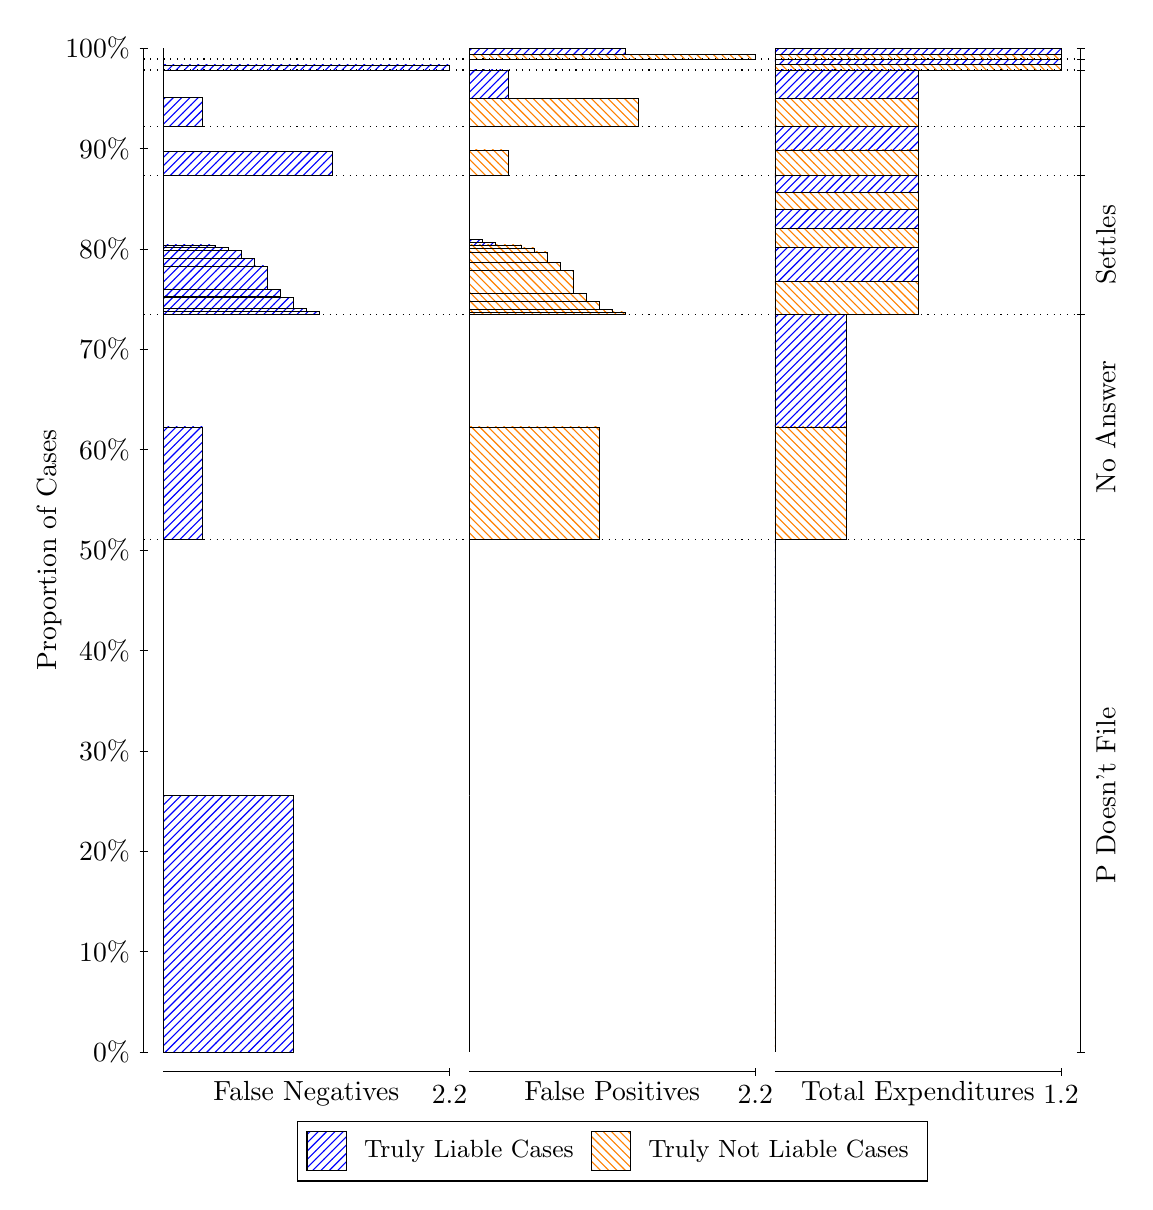
\begin{tikzpicture}
\draw[black, very thin] (1.5,1.75) -- (1.5,14.5);
\node[rotate=90, anchor=center] at (0.3, 8.125) {Proportion of Cases};
\draw[black, very thin] (1.45,1.75) -- (1.55,1.75);
\node[anchor=east] at (1.45, 1.75) {0\%};
\draw[black, very thin] (1.45,3.025) -- (1.55,3.025);
\node[anchor=east] at (1.45, 3.025) {10\%};
\draw[black, very thin] (1.45,4.3) -- (1.55,4.3);
\node[anchor=east] at (1.45, 4.3) {20\%};
\draw[black, very thin] (1.45,5.575) -- (1.55,5.575);
\node[anchor=east] at (1.45, 5.575) {30\%};
\draw[black, very thin] (1.45,6.85) -- (1.55,6.85);
\node[anchor=east] at (1.45, 6.85) {40\%};
\draw[black, very thin] (1.45,8.125) -- (1.55,8.125);
\node[anchor=east] at (1.45, 8.125) {50\%};
\draw[black, very thin] (1.45,9.4) -- (1.55,9.4);
\node[anchor=east] at (1.45, 9.4) {60\%};
\draw[black, very thin] (1.45,10.675) -- (1.55,10.675);
\node[anchor=east] at (1.45, 10.675) {70\%};
\draw[black, very thin] (1.45,11.95) -- (1.55,11.95);
\node[anchor=east] at (1.45, 11.95) {80\%};
\draw[black, very thin] (1.45,13.225) -- (1.55,13.225);
\node[anchor=east] at (1.45, 13.225) {90\%};
\draw[black, very thin] (1.45,14.5) -- (1.55,14.5);
\node[anchor=east] at (1.45, 14.5) {100\%};

\draw[black, very thin] (13.4,1.75) -- (13.4,14.5);
\draw[black, very thin] (13.35,1.75) -- (13.45,1.75);
\node[anchor=west] at (13.35, 1.75) {};
\draw[black, very thin] (13.35,8.2631) -- (13.45,8.2631);
\node[anchor=west] at (13.35, 8.2631) {};
\draw[black, very thin] (13.35,11.114) -- (13.45,11.114);
\node[anchor=west] at (13.35, 11.114) {};
\draw[black, very thin] (13.35,12.886) -- (13.45,12.886);
\node[anchor=west] at (13.35, 12.886) {};
\draw[black, very thin] (13.35,13.509) -- (13.45,13.509);
\node[anchor=west] at (13.35, 13.509) {};
\draw[black, very thin] (13.35,14.221) -- (13.45,14.221);
\node[anchor=west] at (13.35, 14.221) {};
\draw[black, very thin] (13.35,14.36) -- (13.45,14.36);
\node[anchor=west] at (13.35, 14.36) {};
\draw[black, very thin] (13.35,14.5) -- (13.45,14.5);
\node[anchor=west] at (13.35, 14.5) {};

\draw[black, very thin, pattern color=blue, pattern=north east lines] (1.75,1.75) rectangle (3.4015,5.0065);
\draw[black, very thin, pattern color=orange, pattern=north west lines] (1.75,5.0065) rectangle (1.75,8.2631);
\draw[black, very thin, pattern color=blue, pattern=north east lines] (1.75,8.2631) rectangle (2.2455,9.6884);
\draw[black, very thin, pattern color=orange, pattern=north west lines] (1.75,9.6884) rectangle (1.75,11.114);
\draw[black, very thin, pattern color=blue, pattern=north east lines] (1.75,11.114) rectangle (3.7318,11.152);
\draw[black, very thin, pattern color=blue, pattern=north east lines] (1.75,11.152) rectangle (3.5667,11.198);
\draw[black, very thin, pattern color=blue, pattern=north east lines] (1.75,11.198) rectangle (3.4015,11.329);
\draw[black, very thin, pattern color=blue, pattern=north east lines] (1.75,11.329) rectangle (3.2364,11.353);
\draw[black, very thin, pattern color=blue, pattern=north east lines] (1.75,11.353) rectangle (3.2364,11.438);
\draw[black, very thin, pattern color=blue, pattern=north east lines] (1.75,11.438) rectangle (3.0712,11.732);
\draw[black, very thin, pattern color=blue, pattern=north east lines] (1.75,11.732) rectangle (2.9061,11.829);
\draw[black, very thin, pattern color=blue, pattern=north east lines] (1.75,11.829) rectangle (2.7409,11.932);
\draw[black, very thin, pattern color=blue, pattern=north east lines] (1.75,11.932) rectangle (2.5758,11.964);
\draw[black, very thin, pattern color=blue, pattern=north east lines] (1.75,11.964) rectangle (2.4106,12.001);
\draw[black, very thin, pattern color=orange, pattern=north west lines] (1.75,12.001) rectangle (1.75,12.886);
\draw[black, very thin, pattern color=blue, pattern=north east lines] (1.75,12.886) rectangle (3.897,13.19);
\draw[black, very thin, pattern color=orange, pattern=north west lines] (1.75,13.19) rectangle (1.75,13.509);
\draw[black, very thin, pattern color=blue, pattern=north east lines] (1.75,13.509) rectangle (2.2455,13.872);
\draw[black, very thin, pattern color=orange, pattern=north west lines] (1.75,13.872) rectangle (1.75,14.221);
\draw[black, very thin, pattern color=blue, pattern=north east lines] (1.75,14.221) rectangle (5.3833,14.285);
\draw[black, very thin, pattern color=orange, pattern=north west lines] (1.75,14.285) rectangle (1.75,14.36);
\draw[black, very thin, pattern color=orange, pattern=north west lines] (1.75,14.36) rectangle (1.75,14.424);
\draw[black, very thin, pattern color=blue, pattern=north east lines] (1.75,14.424) rectangle (1.75,14.5);
\draw[black, very thin, pattern color=orange, pattern=north west lines] (5.6333,1.75) rectangle (5.6333,5.0065);
\draw[black, very thin, pattern color=blue, pattern=north east lines] (5.6333,5.0065) rectangle (5.6333,8.2631);
\draw[black, very thin, pattern color=orange, pattern=north west lines] (5.6333,8.2631) rectangle (7.2848,9.6884);
\draw[black, very thin, pattern color=blue, pattern=north east lines] (5.6333,9.6884) rectangle (5.6333,11.114);
\draw[black, very thin, pattern color=orange, pattern=north west lines] (5.6333,11.114) rectangle (7.6152,11.149);
\draw[black, very thin, pattern color=orange, pattern=north west lines] (5.6333,11.149) rectangle (7.45,11.18);
\draw[black, very thin, pattern color=orange, pattern=north west lines] (5.6333,11.18) rectangle (7.2848,11.284);
\draw[black, very thin, pattern color=orange, pattern=north west lines] (5.6333,11.284) rectangle (7.1197,11.382);
\draw[black, very thin, pattern color=orange, pattern=north west lines] (5.6333,11.382) rectangle (6.9545,11.675);
\draw[black, very thin, pattern color=orange, pattern=north west lines] (5.6333,11.675) rectangle (6.7894,11.781);
\draw[black, very thin, pattern color=orange, pattern=north west lines] (5.6333,11.781) rectangle (6.6242,11.912);
\draw[black, very thin, pattern color=orange, pattern=north west lines] (5.6333,11.912) rectangle (6.4591,11.961);
\draw[black, very thin, pattern color=orange, pattern=north west lines] (5.6333,11.961) rectangle (6.2939,11.999);
\draw[black, very thin, pattern color=blue, pattern=north east lines] (5.6333,11.999) rectangle (5.9636,12.035);
\draw[black, very thin, pattern color=blue, pattern=north east lines] (5.6333,12.035) rectangle (5.7985,12.067);
\draw[black, very thin, pattern color=blue, pattern=north east lines] (5.6333,12.067) rectangle (5.6333,12.886);
\draw[black, very thin, pattern color=orange, pattern=north west lines] (5.6333,12.886) rectangle (6.1288,13.205);
\draw[black, very thin, pattern color=blue, pattern=north east lines] (5.6333,13.205) rectangle (5.6333,13.509);
\draw[black, very thin, pattern color=orange, pattern=north west lines] (5.6333,13.509) rectangle (7.7803,13.858);
\draw[black, very thin, pattern color=blue, pattern=north east lines] (5.6333,13.858) rectangle (6.1288,14.221);
\draw[black, very thin, pattern color=orange, pattern=north west lines] (5.6333,14.221) rectangle (5.6333,14.296);
\draw[black, very thin, pattern color=blue, pattern=north east lines] (5.6333,14.296) rectangle (5.6333,14.36);
\draw[black, very thin, pattern color=orange, pattern=north west lines] (5.6333,14.36) rectangle (9.2667,14.424);
\draw[black, very thin, pattern color=blue, pattern=north east lines] (5.6333,14.424) rectangle (7.6152,14.5);
\draw[black, very thin, pattern color=orange, pattern=north west lines] (9.5167,1.75) rectangle (9.5167,5.0065);
\draw[black, very thin, pattern color=blue, pattern=north east lines] (9.5167,5.0065) rectangle (9.5167,8.2631);
\draw[black, very thin, pattern color=orange, pattern=north west lines] (9.5167,8.2631) rectangle (10.425,9.6884);
\draw[black, very thin, pattern color=blue, pattern=north east lines] (9.5167,9.6884) rectangle (10.425,11.114);
\draw[black, very thin, pattern color=orange, pattern=north west lines] (9.5167,11.114) rectangle (11.333,11.541);
\draw[black, very thin, pattern color=blue, pattern=north east lines] (9.5167,11.541) rectangle (11.333,11.971);
\draw[black, very thin, pattern color=orange, pattern=north west lines] (9.5167,11.971) rectangle (11.333,12.213);
\draw[black, very thin, pattern color=blue, pattern=north east lines] (9.5167,12.213) rectangle (11.333,12.452);
\draw[black, very thin, pattern color=orange, pattern=north west lines] (9.5167,12.452) rectangle (11.333,12.668);
\draw[black, very thin, pattern color=blue, pattern=north east lines] (9.5167,12.668) rectangle (11.333,12.886);
\draw[black, very thin, pattern color=orange, pattern=north west lines] (9.5167,12.886) rectangle (11.333,13.205);
\draw[black, very thin, pattern color=blue, pattern=north east lines] (9.5167,13.205) rectangle (11.333,13.509);
\draw[black, very thin, pattern color=orange, pattern=north west lines] (9.5167,13.509) rectangle (11.333,13.858);
\draw[black, very thin, pattern color=blue, pattern=north east lines] (9.5167,13.858) rectangle (11.333,14.221);
\draw[black, very thin, pattern color=orange, pattern=north west lines] (9.5167,14.221) rectangle (13.15,14.296);
\draw[black, very thin, pattern color=blue, pattern=north east lines] (9.5167,14.296) rectangle (13.15,14.36);
\draw[black, very thin, pattern color=orange, pattern=north west lines] (9.5167,14.36) rectangle (13.15,14.424);
\draw[black, very thin, pattern color=blue, pattern=north east lines] (9.5167,14.424) rectangle (13.15,14.5);
\draw[black, dotted] (1.5,8.2631) -- (13.4,8.2631);
\draw[black, dotted] (1.5,11.114) -- (13.4,11.114);
\draw[black, dotted] (1.5,12.886) -- (13.4,12.886);
\draw[black, dotted] (1.5,13.509) -- (13.4,13.509);
\draw[black, dotted] (1.5,14.221) -- (13.4,14.221);
\draw[black, dotted] (1.5,14.36) -- (13.4,14.36);
\draw[black, very thin] (1.75,1.5) -- (5.3833,1.5);
\node[anchor=north] at (3.5667, 1.5) {False Negatives};
\draw[black, very thin] (5.3833,1.45) -- (5.3833,1.55);
\node[anchor=north] at (5.3833, 1.45) {2.2};

\draw[black, very thin] (5.6333,1.5) -- (9.2667,1.5);
\node[anchor=north] at (7.45, 1.5) {False Positives};
\draw[black, very thin] (9.2667,1.45) -- (9.2667,1.55);
\node[anchor=north] at (9.2667, 1.45) {2.2};

\draw[black, very thin] (9.5167,1.5) -- (13.15,1.5);
\node[anchor=north] at (11.333, 1.5) {Total Expenditures};
\draw[black, very thin] (13.15,1.45) -- (13.15,1.55);
\node[anchor=north] at (13.15, 1.45) {1.2};

\node[black, centered, rotate=90] at (13.72, 5.0065) {P Doesn't File};
\node[black, centered, rotate=90] at (13.72, 9.6884) {No Answer};
\node[black, centered, rotate=90] at (13.72, 12) {Settles};





\draw (7.449999999999999,1.5) node[draw=none] (baseCoordinate) {};
\begin{scope}[align=center]
        \matrix[scale=0.5, draw=black, below=0.5cm of baseCoordinate, nodes={draw}, column sep=0.1cm]{
            \node[rectangle, draw, minimum width=0.5cm, minimum height=0.5cm, pattern=north east lines, pattern color=blue] {}; &
            \node[draw=none, font=\small] (B) {Truly Liable Cases}; &
            \node[rectangle, draw, minimum width=0.5cm, minimum height=0.5cm, pattern=north west lines, pattern color=orange] {}; &
            \node[draw=none, font=\small] (B) {Truly Not Liable Cases}; \\
            };
\end{scope}

\end{tikzpicture}
\end{document}